\documentclass[12pt,a4paper]{report}
\usepackage{graphicx}
\usepackage{color}
\usepackage{newtxtext,newtxmath}
\usepackage{bm}
\usepackage[hidelinks]{hyperref}
\usepackage{natbib}
\bibliographystyle{agu08}

\usepackage{listings}


\lstdefinestyle{myMATLAB}{ %
language=MATLAB,                % choose the language of the code
basicstyle=\footnotesize\ttfamily,       % the size of the fonts that are used for the code
%numbers=left,                   % where to put the line-numbers
%numberstyle=\footnotesize\ttfamily,      % the size of the fonts that are used for the line-numbers
%stepnumber=1,                   % the step between two line-numbers. If it is 1 each line will be numbered
%numbersep=5pt,                  % how far the line-numbers are from the code
backgroundcolor=\color{white},  % choose the background color. You must add \usepackage{color}
showspaces=false,               % show spaces adding particular underscores
showstringspaces=false,         % underline spaces within strings
showtabs=false,                 % show tabs within strings adding particular underscores
%frame=false,           % adds a frame around the code
tabsize=4,          % sets default tabsize to 2 spaces
captionpos=b,           % sets the caption-position to bottom
breaklines=false,        % sets automatic line breaking
breakatwhitespace=false,    % sets if automatic breaks should only happen at whitespace
%escapeinside={\%*}{*)},          % if you want to add a comment within your code
commentstyle=\footnotesize\color{blue},
xleftmargin=0pt,
columns=flexible
}


\lstdefinestyle{myMATLABsmall}{ %
language=MATLAB,                % choose the language of the code
basicstyle=\tiny\ttfamily,       % the size of the fonts that are used for the code
%numbers=left,                   % where to put the line-numbers
%numberstyle=\footnotesize\ttfamily,      % the size of the fonts that are used for the line-numbers
%stepnumber=1,                   % the step between two line-numbers. If it is 1 each line will be numbered
%numbersep=5pt,                  % how far the line-numbers are from the code
backgroundcolor=\color{white},  % choose the background color. You must add \usepackage{color}
showspaces=false,               % show spaces adding particular underscores
showstringspaces=false,         % underline spaces within strings
showtabs=false,                 % show tabs within strings adding particular underscores
%frame=false,           % adds a frame around the code
tabsize=4,          % sets default tabsize to 2 spaces
captionpos=b,           % sets the caption-position to bottom
breaklines=false,        % sets automatic line breaking
breakatwhitespace=false,    % sets if automatic breaks should only happen at whitespace
%escapeinside={\%*}{*)},          % if you want to add a comment within your code
commentstyle=\footnotesize\color{blue},
xleftmargin=0pt,
columns=flexible
}


\title{ELSPEC \\
\author{Ilkka Virtanen\\
Ionospheric Physics research unit\\ University of Oulu, Finland}
\date{Version 0.1 \\ \today}                                           % Activate to display a given date or no date
}
\begin{document}
\sloppy

%%\begin{fullpage}
\maketitle
%%\end{fullpage}



\newpage

\chapter*{License}
{\small

{\bfseries ElSpec}
\vspace*{6pt}

\noindent \texttt{Copyright 2015-2018 Ilkka Virtanen and Bj{\"o}rn Gustavsson}
\vspace*{6pt}

\begin{verbatim}
This program is free software; you can redistribute it and/or
modify it under the terms of the GNU General Public License
as published by the Free Software Foundation; either version 2
of the License, or (at your option) any later version.

This program is distributed in the hope that it will be useful,
but WITHOUT ANY WARRANTY; without even the implied warranty of	
MERCHANTABILITY or FITNESS FOR A PARTICULAR PURPOSE.  See the
GNU General Public License for more details.

You should have received a copy of the GNU General Public License
along with this program; if not, write to the Free Software
Foundation, Inc., 51 Franklin Street, Fifth Floor, Boston, MA  02110-1301, USA.
\end{verbatim}
}




\newpage


\tableofcontents

\newpage




\chapter{Introduction}

\section{ElSpec}

ELSPEC is a MATLAB toolbox for estimating differential energy flux of precipitating electrons from field-aligned EISCAT incoherent scatter radar observations of ionospheric electron density. The ELSPEC input data are analysis results from the standard EISCAT data analysis tool, GUISDAP. The input data may be GUISDAP raw densities, GUISDAP fit results, or both. %The software assumes that the radar is in magnetic field-aligned position.
Electron density profiles from other than field-aligned directions are automatically excluded from the analysis. Several different models of ion production, recombination, and ion composition are available. Also time-resolution and energy grid points can be selected by the user, the former within the limits set by EISCAT experiment design. 


ELSPEC is an upgraded version of the electron energy spectrum estimation technique developed by Bj{\"o}rn Gustavsson, which was used in \citep{dahlgren2011}. The upgraded technique and validation results are published in \citep{virtanen2018}

\section{System requirements}

ELSPEC has been run on Linux with MATLAB2021b and earlier versions. Other reasonably recent MATLAB versions and other operating system will probably work as well. 

ELSPEC uses the MATLAB implementations of the NRLMSISE-00 model (atmosnrlmsise00) and IGRF (igrfmagm) in the Aerospace toolbox. This version of ELSPEC cannot be used without the Aerospace toolbox. 

\section{Installation}

ELSPEC is distributed as a MATLAB toolbox. Add full path to the 'ELSPEC' directory in your MATLAB search path or, if you received the package as an .mltbx-file, install it using the MATLAB toolbox installer (a double-click is typically enough).


\section{Help}\label{help}

Standard MATLAB help messages are available at least for the user interface functions. Full command references for the main inversion and plotting routines are given in Appendix \ref{chapCommands} of this document. 


\section{Reference}

In published scientific works using ELSPEC, please refer to the paper:

Ilkka I. Virtanen, Bj{\"o}rn Gustavsson, Anita Aikio, Antti Kero, Kazushi Asamura, and Yasunobu Ogawa, Electron energy spectrum and auroral power estimation from incoherent scatter radar measurements, J. Geophys. Res. Space Physics, 123, 6865-6887, 2018, \href{https://doi.org/doi:10.1029/2018JA025636}{doi:10.1029/2018JA025636}.
%Ilkka I. Virtanen, Bj{\"o}rn Gustavsson, Anita Aikio, Antti Kero, Kazushi Asamura and Yasunobu Ogawa, Incoherent scatter observations of electron precipitation energy flux in the auroral ionosphere, J. Geophys. Res. Space Physics, ....


\chapter{Electron energy spectrum estimation}

The electron energy spectrum inversion is shortly outlined in this chapter. See \cite[][and references therein]{virtanen2018} for details. 

\section{Electron precipitation and ion production}

Energetic electrons precipitating to the ionosphere cause collisional ionization. If plasma convection and photoionization can be neglected, the electron gas will follow the continuity equation
\begin{equation}
\frac{\partial N}{\partial t} = Q + \alpha N^2,
\label{eqContinuity}
\end{equation}
where $N$ is the electron number density, $t$ is time  and $Q$ is electron production rate per unit volume.

The ion production rate depends on composition of the neutral atmosphere and the differential number flux of the precipitating electrons. If the neutral atmosphere is known, $Q$ can be calculated for arbitrary electron fluxes and altitudes. Similarly, if the ion composition is known, the effective recombination coefficient $\alpha$ can be calculated. 

Incoherent scatter radars can observe electron density as function of time and altitude along a geomagnetic field-line. At night the assumptions of negligible photoionization and plasma convection are reasonable in the E region. Because the ion production rate can be expressed as a function of the differential number flux $I$, $Q=Q(I(t))$, the differential number flux can be inverted from the incoherent scatter radar data.



\section{ELSPEC implementation}

Key points of the ELSPEC inversion are \emph{analytic integration of the electron continuity equation}, \emph{fits with multiple models} of the spectrum shape, and \emph{model selection} by means of the Akaike information criterion. These are shortly outlined below. 

\subsection{Integration of the electron continuity equation}

Input data to ELSPEC are vectors of electron density at discrete height-gates $h_i$, sampled at times $t_j$, 
\begin{equation}
\bm{N}_j = \left(
\begin{array}{c}
N_{j,1}\\
N_{j,2}\\
\vdots \\
N_{j,H}
\end{array}
\right),
\end{equation}
where $H$ is the number of height gates. 

Ion production rate in each gate are calculated as matrix product
\begin{equation}
\bm{Q}_j = \bm{A}\bm{I}_j,
\end{equation}
where $\bm{Q}_j$ is a vector of ion production rates, elements of the matrix $\bm{A}$ are calculated using an ion production model, and $\bm{I}_j$ is the differential number flux. In a similar manner, the effective recombination coefficients in each height gate are collected in a vector
\begin{equation}
\bm{\alpha}_j = \left(
\begin{array}{c}
\alpha_{j,1}\\
\alpha_{j,2}\\
\vdots\\
\alpha_{j,H}
\end{array}
\right).
\end{equation}


A key point in the ELSPEC implementation is that the time-derivative of electron density $\partial N / \partial t$ is not explicitly calculated from data, but the software makes an iterative search to find the differential number flux $\bm{I}$ that leads to best match between the observed electron density and the analytic solution from Equation (\ref{eqContinuity}). Electron density as function of time, as solved from (\ref{eqContinuity}), is
\begin{equation}
n(t) = \frac{ n(t_{j-1}) + \sqrt{Q_j/ \alpha_j}\tanh\left(\sqrt{\alpha_j Q_j} t\right) }{ 1 + \sqrt{\alpha_kQ_j}n(t_{j-1})\tanh\left(\sqrt{\alpha_j Q_j} t\right)} \quad, t_{j-1}\leq t \leq t_{j}.
\label{eqNet}
\end{equation}
Here $n(t)$ is the electron density and $n(t_{j-1})$ is the density at beginning of the current time step. Because the radar observations are averages over a time step, the model values, which should match with the observed densities, are integrated from (\ref{eqNet}),
%\begin{eqnarray}
%n_k = &\frac{ 1}{ \Delta t}\left(\frac{\log{\left( \sqrt{Q_j} + \sqrt{\alpha_j}n(t_{j-1})\tanh{\left(\sqrt{\alpha_j Q_j}\Delta t\right)}\right)} - \log\left(\tanh\left(\sqrt{\alpha_j Q_j}\Delta t\right) + 1\right) + \sqrt{\alpha_j Q_j}\Delta t}{\alpha_j}  -\log\left(\sqrt{Q_j}\right)\alpha_j\right).\nonumber \\
%&
%\label{eqDirthe}
%\end{eqnarray}
\begin{equation}
\mathbf{n}_k=
\frac{1}{\mbox{\boldmath{$\alpha$}}_k \Delta t}
\left(
\log\left(
\frac{\mathbf{n}(t_{k-1})\sqrt{\mbox{\boldmath{$\alpha$}}_k/\mathbf{Q}_k}\tanh\left(\sqrt{\mbox{\boldmath{$\alpha$}}_k\mathbf{Q}_k}\Delta t\right)+1}{\tanh\left(\sqrt{\mbox{\boldmath{$\alpha$}}_k\mathbf{Q}_k}\Delta t\right) + 1}
\right)
+\sqrt{\mbox{\boldmath{$\alpha$}}_k\mathbf{Q}_k}\Delta t
\right).
\label{eqDirthe}
\end{equation}


\subsection{Spectrum models}

The inverse problem in electron energy spectrum estimation is ill-posed in general, because large energy interval needs to be covered with rather high resolution, but typically only some tens of electron density observations are available for each time step. Regularizing information is thus needed, and this information is included in the form of parametric spectrum shape models in ELSPEC. 

There is a variety of models one could potentially use. For example, Maxwellian and $\kappa$ distributions, as well as narrow- and wide-band accelerated spectra  are observed by satellites above and within the ionosphere. The original implementation in \cite{dahlgren2011} used an exponential of a spline expansion, with both the spline node locations and their amplitudes determined in the inversion. 

ELSPEC uses a slightly different polynomial model, because the model of \cite{dahlgren2011} reduces to a polynomial when number of spline nodes is small, which is almost always the case, and the polynomials are technically somewhat easier to control. The polynomial model is of the form
\begin{equation}
I = \bm{E}\exp{\left(\sum_{l=0}^L{P_L(l)\bm{E}^l}\right)},
\end{equation}
where $P_L$ is a vector of $L+1$ polynomial coefficients, which are the unknowns in the inversion. The vector $\bm{E}$ is the selected energy grid. The model can produce exact Maxwellian fluxes, as well as slightly distorted ones with $L=1$, and more complex shapes, such as $\kappa$ distributions, with higher $L$.

\subsection{Model selection}

On each time-step, ELSPEC runs a separate fit for each spectrum shape model with $L=1,2,\ldots,N_{max}$, where $N_{max}$ is typically between 5 and 10. The optimal one, which is then selected as the final estimate of the differential number flux, is then selected by means of the Akaike information criterion \citep[e.g.][]{burnham2002}.


\subsection{Error estimation}

Error estimation in ELSPEC is somewhat complicated, because the error in the modeled electron density in beginning of the integration must be taken into account. An error estimation based on an assumption of Gaussian error distributions and numerical derivatives of linearized theory in vicinity of the iteration convergence point is implemented. 

\subsection{Derived parameters}

Several derived parameters and their error estimates are calculated from the differential number flux estimates $\bm{I}_j$ and their covariances. 

~

\noindent{\bf Differential energy flux} is calculated as a product of the differential number flux and the known energy grid values. 

~

\noindent{\bf Upward field aligned current} carried by the precipitating electrons is integrated from the differential number flux. However, this estimate might not reflect the true field-aligned current, because ELSPEC cannot see either upward moving electrons or low-energy electrons (typically below 1~keV), whose contribution to the net current may be significant.

~

\noindent{\bf Auroral power} (integral energy flux) of the precipitation is integrated from the differential energy flux. These estimates are accurate, because contribution of the low-energy electrons is very small. The auroral power estimates have been found to be very accurate even if the shape of the differential energy flux is not. 





\chapter{ELSPEC in practice}

The user interface to the ELSPEC inversion is the function \verb|ElSpec|, which can be called with various optional parameters. The parameters, their default values, and examples of their use are listed in Appendix \ref{chapCommands}. This chapter explains most important parts of the analysis in more detail. 


\section{The simplest example}

The simplest, but typically suboptimal way to use ELSPEC is to use standard fitted GUISDAP analysis results as input. Because the default setting are for EISCAT UHF beata experiment, more or less reasonable results will be produced if one cd's to a GUISDAP output directory of any field-aligned (CP1) UHF beata experiment and runs the command
\begin{lstlisting}[style=myMATLAB]
>> ElSpecOut = ElSpec('fitdir','.');
\end{lstlisting}
The software will print its settings, including the output file name. The output file contains a MATLAB struct 'ElSpecOut', where all settings and the inversion results are stored. The same structure is returned by the function when the analysis is complete.  The results can be visualized with the function 'ElSpecPlot'. In the simplest case a plot is produced with the command
\begin{lstlisting}[style=myMATLAB]
>> ElSpecPlot(ElSpecOut);
\end{lstlisting}



\section{Input data}

ELSPEC can use two kinds of EISCAT data as input, 'normal' GUISDAP fit results and high-resolution 'raw densities' from two specific experiments, UHF beata and arc1.  The GUISDAP options for calculating the sufficient raw densities are given in Section \ref{secGUISDAP}. The different input options are explained in the following three subsections. 

\subsection{Both ppdir and fitdir are defined}

If both \verb|ppdir| and \verb|fitdir| are given in the \verb|ElSpec| function call, the electron density data are read from raw electron densities in \verb|ppdir|. Electron temperatures are extracted from the fit results in  \verb|fitdir|. 

In this case the \verb|tres| argument is effective and has two alternatives. \verb|dump| means that the raw densities from EISCAT data dumps are integrated together. Standard deviation of the electron density is calculated as a sample average over all raw density profiles in a data dump. \verb|best| means that the original, best available time resolution is maintained. The same standard deviations are copied for all raw density profiles in each EISCAT data dump. 

This combination is currently available only for EISCAT UHF 'beata' and 'arc1' experiments. 

\subsection{Only fitdir is defined}

If only \verb|fitdir| is defined but \verb|ppdir| is not, ELSPEC reads both electron densities and electron temperatures from the same GUISDAP fit files. This option works with all EISCAT experiments, because the fit results are in a standard format. 

Notice that temperature estimation is typically not possible with very high time resolutions. If GUISDAP is set to fit only electron densities, the temperatures in GUISDAP output files will be from the IRI model. 


\subsection{Only ppdir is defined}

If only \verb|ppdir| is defined, ELSPEC uses the raw electron densities in \verb|ppdir| and takes the electron temperature from a model. Depending on the selected ion recombination model, this model is either IRI or MSIS. In the latter case, electron temperature is assumed to be equal to the neutral temperature. 

The electron temperature is taken from the IRI model if it is needed for the recombination model. Recombination models (\verb|recombmodel|) using IRI are \verb|'Rees'|, \verb|'SheehanGr'| and \verb|'SheehanEx'| (the last one is probably not useful in practice).

This option is available only for EISCAT UHF 'beata' and 'arc1' experiments. 


\section{Running the GUISDAP analysis}\label{secGUISDAP}

GUISDAP default options are sufficient for calculating the normal fit results in \verb|fitdir|. However, one should carefully calibrate the data, because the energy spectrum is a nonlinear function of the density, and calibration errors may have significant, nontrivial effects to the spectrum estimates. 

In order to calculate the raw electron density estimates in \verb|ppdir|, one should use the GUISDAP settings
\begin{verbatim}
analysis_ppshortlags=1
analysis_pponly=1
a_satch.do=0 
\end{verbatim}
The last one disables the GUISDAP satellite echo detection, which may sometimes cause problems with very high time resolutions. The analysis can be run also with the satellite check, but ELSPEC cannot read in data files with data points missing due to satellite echo detections, and such files have to be manually removed. In addition, the analysis time-resolution should be matched with the EISCAT dump length, which is 4~s for UHF arc1 and 5~s for UHF beata. With these options the analysis does not produce the standard fitted parameters at all, but stores only the raw densities with highest available resolutions. ELSPEC provides input routines for reading the experiment-specific GUISDAP outputs for UHF beata and arc1. 

Power calibration is most practical for the standard fit results. The 'magic constant' estimated with the standard fit can (and should) be used also for the raw density fits. 

\section{Ion production models}

ELSPEC allows the user to select between two alternative ion production models. The first implementation used in \cite{dahlgren2011} used an ion production model by \citep{sergienko1993}, which can be selected with the \verb|ionomodel| parameter. The default model is from a more recent work by \citep{fang2010}. 


\section{Ion recombination models}

The effective recombination coefficient $\alpha$ may be an issue in the energy spectrum inversion, because the coefficient depends on two poorly known things, the ion composition and the recombination coefficients of individual ion species. 

The default choice is to use recombination speeds for ions in vibrational ground state from laboratory measurements \citep{sheehan2004} and assume that only NO$^+$ and O$_2^+$ ions, whose abundances are taken from IRI, are present.  The recombination coefficients are different from e.g. the widely used values by \cite{rees1989}, who did not provide different values for the vibrationally excited states. Although there is no practical means to monitor the vibrational state of the molecular ions, the excited states are short-lived in comparison to the ion recombination times, and wast majority of the ions should be in ground state. 

The IRI compositions are known to be suboptimal, because the collisional ionization produces large amounts of O$_2^+$, whose contribution varies rapidly along changes in the precipitation flux. The incorrect compositions have been found to cause up to 30~\% error in the net power flux estimates. In order to provide simpler models, which may be equally good in practice, the package contains options for assuming pure NO$^+$ or pure $O_2^+$ ionospheres. 

Altogether nine different options for the ion recombination model are currently available. These are listed in Appendix \ref{chapCommands}.

\section{Time resolution}

ELSPEC contains a build-in system for controlling the time-resolution according to ionospheric conditions. When electron density is high and recombination fast, the time resolution will automatically drop to the shortest one allowed by the data. When the recombination is slow the user can allow ElSpec to fit to longer periods fo data. The time resolution is determined for each time step and altitude separately, meaning that e.g. low densities at the upper E region may be analyzed with a coarser time resolution than the E region peak. 

The adaptation to the recombination time is built in the system and cannot be directly accessed by the user. The adaptation is based on scaling the electron density variances according to the recombination time-scale, as explained in \cite{virtanen2018}. 

However, the user can control the maximum amount of data used in each fit with the \verb|ninteg| parameter. If this parameter is set to one, the adaptation is disabled and data from exactly one time step is always used. 


\chapter{Examples}

This chapter provides some practical examples of using ELSPEC. 

\section{UHF beata with raw densities}

\begin{figure}[ht]
\begin{center}
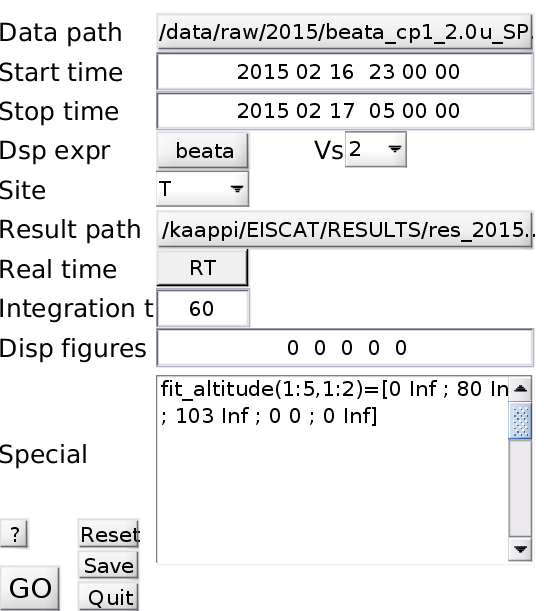
\includegraphics[width=.49\textwidth]{guisdap1.png}
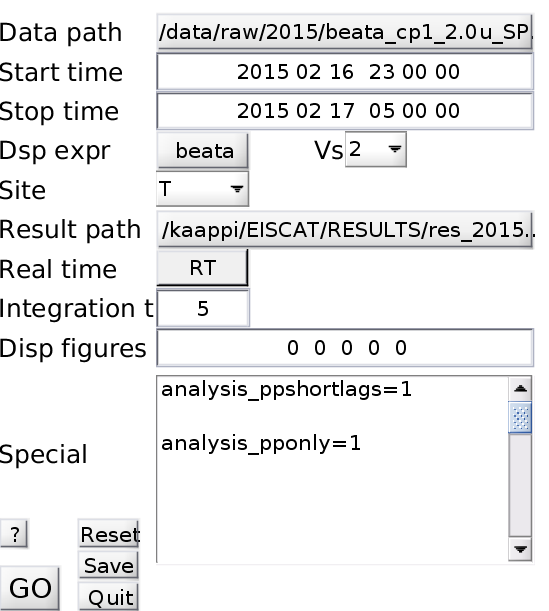
\includegraphics[width=.49\textwidth]{guisdap2.png}
\caption{Left: A GUISDAP GUI window with settings for a fit, which will produce the electron temperature estimates for ELSPEC. Right: A GUISDAP GUI window with setting for a fit of the raw electron densities.}
\label{figGUISDAP}
\end{center}
\end{figure}



\begin{figure}[ht]
\begin{center}
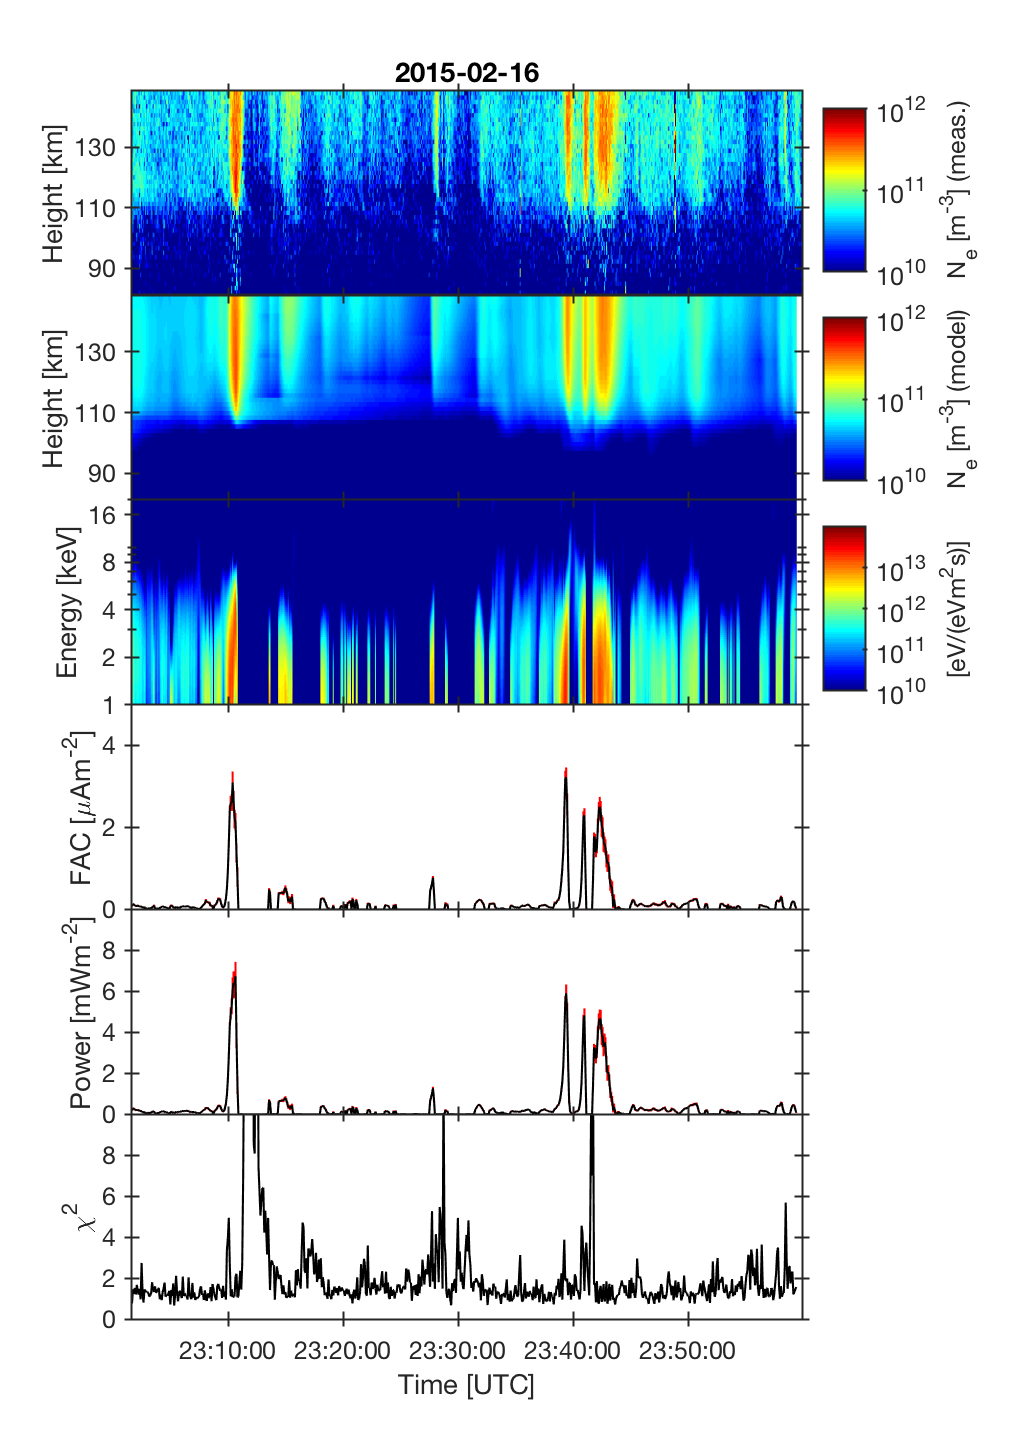
\includegraphics[width=\textwidth]{ElSpec_20150216T230135-20150216T235955_beata_uhf_Fang_SheehanGr_integrate_6_1_dump.png}
\caption{ELSPEC inversion results with the time dependent model and 5~s time resolution. }
\label{figElSpecOut}
\end{center}
\end{figure}

\begin{figure}[ht]
\begin{center}
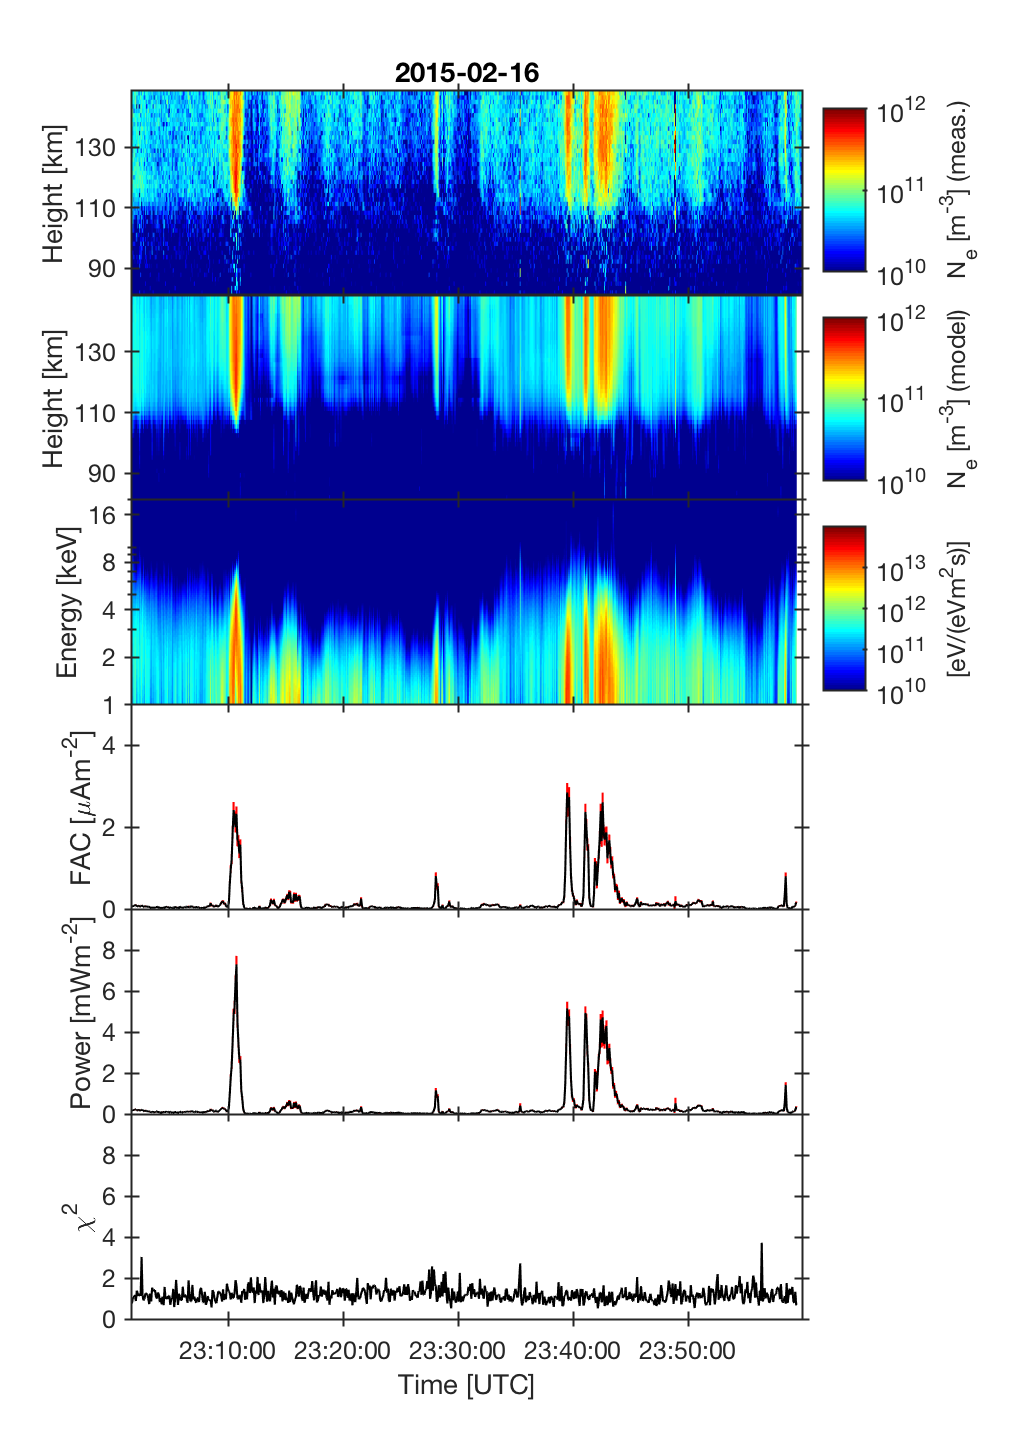
\includegraphics[width=\textwidth]{ElSpec_20150216T230135-20150216T235955_beata_uhf_Fang_SheehanGr_equilibrium_6_1_dump.png}
\caption{ELSPEC inversion results with the steady state model and 5~s time resolution. }
\label{figElSpecOutEquilibrium}
\end{center}
\end{figure}

\begin{figure}[ht]
\begin{center}
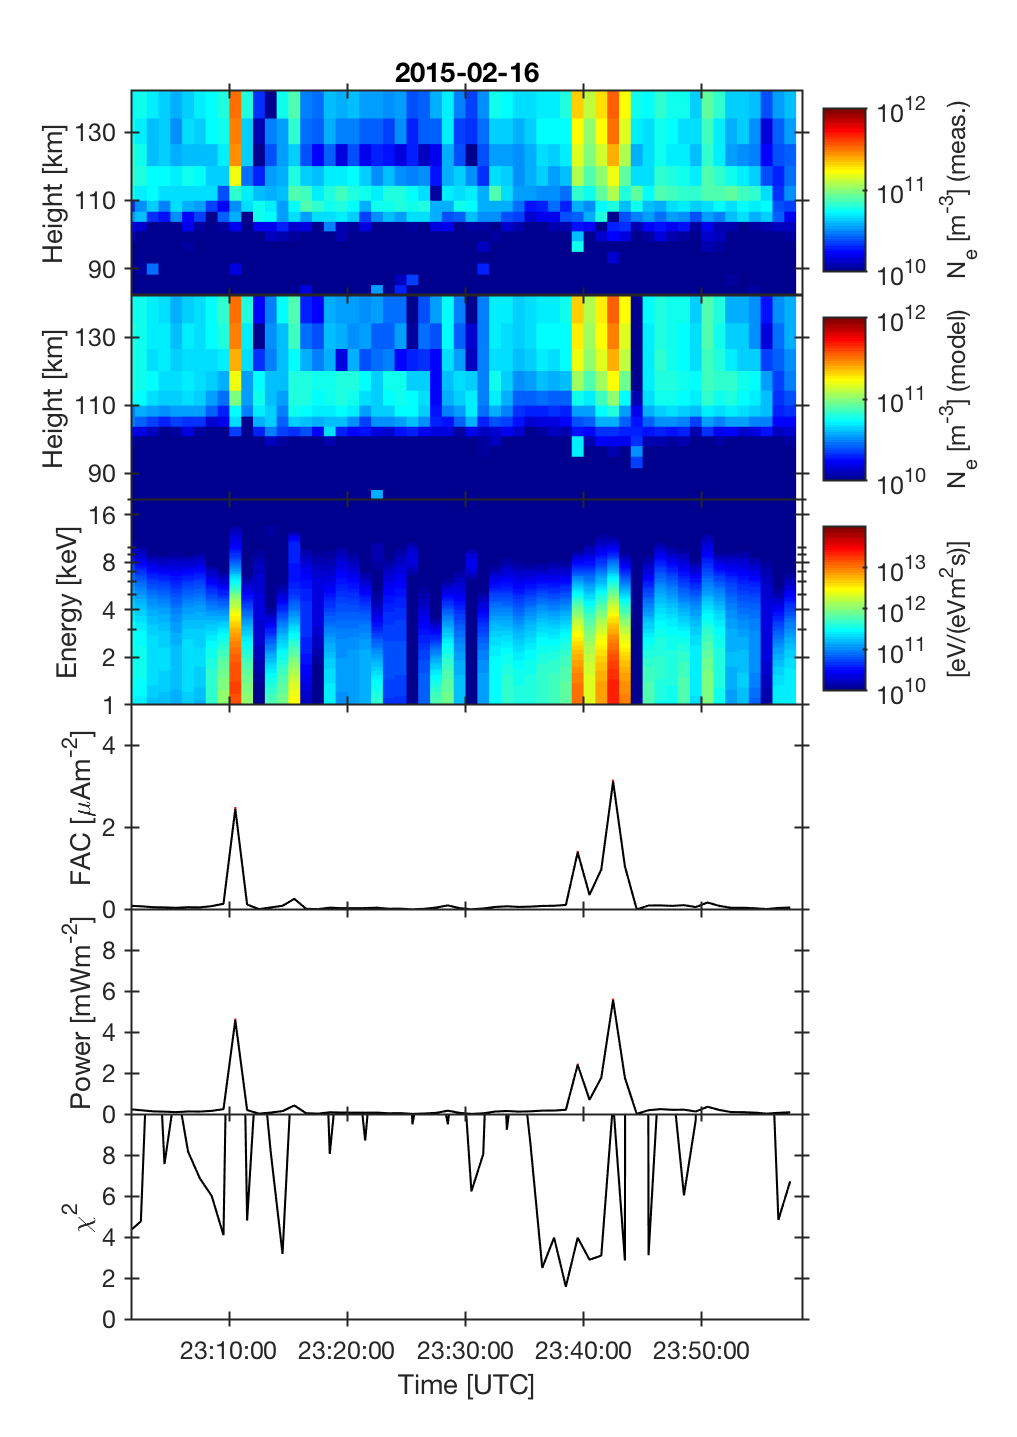
\includegraphics[width=\textwidth]{ElSpec_20150216T230130-20150216T235900_beata_uhf_Fang_SheehanGr_equilibrium_1_1_dump.png}
\caption{ELSPEC inversion results with the steady state model and 60~s time resolution using only the standard GUISDAP fit results.}
\label{figElSpecOutEquilibrium60s}
\end{center}
\end{figure}

A default ELSPEC use case is inversion of EISCAT UHF beata data, using both GUISDAP fits of all plasma parameters and raw electron densities. 

First of all, a 'normal' GUISDAP fit with a rather coarse time resolution is needed. 60~s is typically enough for reasonable temperature estimation. The default height limits for temperature estimation are typically a bit high, and better electron temperature and density estimates can be gained if ion temperature is fitted above 80~km and the electron-to-ion temperature ratio above 103~km. The limits can be set with the GUISDAP \verb|fit_altitude| option. An example of a GUISDAP GUI is given on the left panel of Figure \ref{figGUISDAP}.

After running the analysis, one should carefully calibrate the data, using either plasma lines or comparisons with the EISCAT dynasonde. For example, the dynasonde calibration can be done with the standard GUISDAP function \verb|calib_ne|. Notice that ELSPEC is typically used in conditions, where E region may have strong ionization but the F region is empty, so it may be better to calibrate against the E region peak densities. Also, the dynasonde calibration should be made with a time period where the ionosphere is more or less stable. Another option is to use the plasma line data in beata, which is often available because the electron precipitation heats the electron gas. The plasma lines have the benefit that they are from the very same volume with the ion line data. 

The calibration will suggest a 'Magic constant'. If the value is different from that used in the original analysis, the analysis should be run again with the correct magic constant. The calibration should be checked again after the second analysis run, but is typically OK at this point. If not, one more analysis run might be needed. 

When the data are correctly calibrated, high-resolution raw densities should be calculated from the same data. This is done by means of setting 
\begin{verbatim}
analysis_ppshortlags=1
analysis_pponly=1
a_satch.do=0
\end{verbatim}
in GUISDAP, and selecting a time resolution that matches with the EISCAT data dump length. In UHF beata the resolution is 5~s. An example of a GUISDAP GUI with sufficient settings is given on the right in Figure \ref{figGUISDAP}.

After the GUISDAP analysis, we will have the 60~s fitted parameters and the 5~s raw densities in separate directories. In this case the directories are \verb|2015-02-16_beata_60s@uhfa| and \verb|2015-02-16_beata_5_rawNe@uhfa|. Because the \verb|ElSpec| defaults are for the UHF beata experiment, we can start the inversion by means of providing only the data directories,


\begin{lstlisting}[style=myMATLAB]
>> out=ElSpec('ppdir','2015-02-16_beata_5_rawNe@uhfa','fitdir','2015-02-16_beata_60@uhfa');
\end{lstlisting}

ELSPEC will then print the license information\footnote{Only on the first call in each MATLAB session} and its settings. The listing is worth checking, especially when analyzing other EISCAT experiments than the default beata, to be sure that all default parameters match with the experiment at hand. \verb|ElSpec| reads all input data at once, which may take some time. When all data are read the result file name is printed, and information about each time step is printed while the inversion proceeds. An example of the output is given below. 



\begin{lstlisting}[style=myMATLABsmall]
>> out = ElSpec('ppdir','2015-02-16_beata_5_rawNe@uhfa','fitdir','2015-02-16_beata_60@uhfa')
  
Copyright 2015-2018, Ilkka Virtanen and Bjorn Gustavsson
This is free software, licensed under GNU GPL version 2 or later.
  
This program is distributed in the hope that it will be useful, 
but WITHOUT ANY WARRANTY; without even the implied warranty of 
MERCHANTABILITY or FITNESS FOR A PARTICULAR PURPOSE.
See the GNU General Public License for more details

ElSpec input arguments

       ppdir: 2015-02-16_beata_5_rawNe@uhfa
      fitdir: 2015-02-16_beata_60@uhfa
  experiment: beata
       radar: uhf
     version: 1
   hmin [km]:  80.0
   hmax [km]: 150.0
       btime: 
       etime: 
   ionomodel: Fang
 recombmodel: SheehanGr
   integtype: integrate
     E [keV]:   0.01  0.01  0.01  0.01  0.01  0.01  0.01  0.01  0.01  0.01
                0.01  0.01  0.01  0.01  0.02  0.02  0.02  0.02  0.02  0.02
                0.02  0.02  0.02  0.02  0.02  0.02  0.02  0.02  0.02  0.02
                0.03  0.03  0.03  0.03  0.03  0.03  0.03  0.03  0.03  0.03
                0.03  0.04  0.04  0.04  0.04  0.04  0.04  0.04  0.04  0.05
                0.05  0.05  0.05  0.05  0.05  0.05  0.06  0.06  0.06  0.06
                0.06  0.07  0.07  0.07  0.07  0.07  0.08  0.08  0.08  0.08
                0.09  0.09  0.09  0.09  0.10  0.10  0.10  0.11  0.11  0.11
                0.12  0.12  0.13  0.13  0.13  0.14  0.14  0.15  0.15  0.16
                0.16  0.16  0.17  0.18  0.18  0.19  0.19  0.20  0.20  0.21
                0.22  0.22  0.23  0.24  0.25  0.25  0.26  0.27  0.28  0.29
                0.30  0.31  0.32  0.32  0.34  0.35  0.36  0.37  0.38  0.39
                0.40  0.42  0.43  0.44  0.46  0.47  0.48  0.50  0.52  0.53
                0.55  0.57  0.58  0.60  0.62  0.64  0.66  0.68  0.70  0.72
                0.75  0.77  0.79  0.82  0.84  0.87  0.90  0.93  0.95  0.98
                1.02  1.05  1.08  1.11  1.15  1.18  1.22  1.26  1.30  1.34
                1.38  1.43  1.47  1.52  1.56  1.61  1.66  1.71  1.77  1.82
                1.88  1.94  2.00  2.06  2.13  2.19  2.26  2.33  2.41  2.48
                2.56  2.64  2.72  2.81  2.89  2.98  3.08  3.17  3.27  3.38
                3.48  3.59  3.70  3.82  3.94  4.06  4.19  4.32  4.45  4.59
                4.74  4.89  5.04  5.20  5.36  5.53  5.70  5.88  6.06  6.25
                6.45  6.65  6.86  7.07  7.29  7.52  7.76  8.00  8.25  8.51
                8.77  9.05  9.33  9.62  9.92 10.23 10.55 10.88 11.22 11.58
               11.94 12.31 12.70 13.09 13.50 13.93 14.36 14.81 15.27 15.75
               16.24 16.75 17.28 17.82 18.37 18.95 19.54 20.15 20.78 21.43
               22.10 22.80 23.51 24.24 25.00 25.79 26.59 27.42 28.28 29.17
               30.08 31.02 31.99 32.99 34.02 35.09 36.18 37.32 38.48 39.69
               40.93 42.21 43.53 44.89 46.30 47.75 49.24 50.78 52.37 54.01
               55.70 57.44 59.23 61.09 63.00 64.97 67.00 69.10 71.26 73.49
               75.79 78.16 80.60 83.13 85.73 88.41 91.17 94.03 96.97 100.00
    maxorder: 5
     plotres: 1
        tres: dump
   Emin [eV]:       1000
      ninteg: 6
       nstep: 1
Will write results in:
 ElSpec_20150216T230135-20150216T235955_beata_uhf_Fang_SheehanGr_integrate_6_1_dump_20180221T123708.mat
16-Feb-2015 23:01:37 4 order, chisqr: 0.8, FAC:  0.08 ( 0.01) muA/m^2, Power:  0.19 ( 0.02) mW/m^2
16-Feb-2015 23:01:42 1 order, chisqr: 1.5, FAC:  0.13 ( 0.02) muA/m^2, Power:  0.29 ( 0.04) mW/m^2
16-Feb-2015 23:01:47 1 order, chisqr: 1.2, FAC:  0.12 ( 0.02) muA/m^2, Power:  0.28 ( 0.04) mW/m^2
16-Feb-2015 23:01:52 1 order, chisqr: 1.5, FAC:  0.09 ( 0.02) muA/m^2, Power:  0.22 ( 0.04) mW/m^2
16-Feb-2015 23:01:57 1 order, chisqr: 1.2, FAC:  0.08 ( 0.01) muA/m^2, Power:  0.21 ( 0.04) mW/m^2
16-Feb-2015 23:02:02 1 order, chisqr: 1.7, FAC:  0.08 ( 0.02) muA/m^2, Power:  0.20 ( 0.04) mW/m^2

\end{lstlisting}

With the default settings ELSPEC will regularly update a plot of the inversions results, and will leave a plot of the final results open when the analysis is finished. The default axis limits used in this plot may not be the optimal ones. In this case we adjust the axis limits with
\begin{lstlisting}[style=myMATLAB]
>> ElSpecPlot(out,'plim',[0 10],'faclim',[0 5],'elim',[1 20]);
\end{lstlisting}

The plot produced with this command is shown in Figure \ref{figElSpecOut}. The top panel is the observed raw electron density, followed by the density modeled in the inversion, the inverted differential energy flux, the upward field-aligned current, and the net energy flux. The bottom panel is $\chi^2$ of the fit. 

Figure \ref{figElSpecOut} shows a relatively good match between the observed and modeled densities, but also reveals one key issue in the inversion. Clearly visible mismatch between the model and the observation is seen during sudden decreases in electron density around 23:11, 23:15, 23:28, etc., where the ELSPEC recombination model does not allow the electrons to recombine as fast as the density decreases in the observed data. These issues are possibly related to ion convection -- the plasma may have moved out of the radar beam instead of recombining within the beam. 

\section{UHF beata with a steady state model}

The steady state assumption, i.e. the assumption that ion production and recombination are in balance during an analysis time step, is widely used in electron energy spectrum inversion. This option can be selected with the \verb|integtype| option of ELSPEC. The same beata data can be analyzed with the steady state assumption using the command
\begin{lstlisting}[style=myMATLAB]
out=ElSpec('ppdir','2015-02-16_beata_5_rawNe@uhfa','fitdir', ...
             '2015-02-16_beata_60@uhfa','integtype','equilibrium');
\end{lstlisting}

Result of this inversion shown in Figure \ref{figElSpecOutEquilibrium}. A clear difference to the result with time dependet model in Figure \ref{figElSpecOut} is that the issue with rapidly decreasing electron densities is not visible. The steady state model finds a precipitation, which would lead to the observed density profile if the energy spectrum remained unchanged for a long period of time. Individual time steps are thus completely independent and the analysis has no problem to adjust to arbitrarily large changes in the electron density. However, the steady state assumption is implicitly wrong and the smoother result is by no means better than the time dependent model -- the simplistic steady state model simply hides the issue.

\section{A fast inversion with fitted data}

A simple way to create quicklook plots that give a rough idea of the energy spectrum characteristics is to run the inversion with standard GUISDAP fit results alone. Such an inversion is very fast to run and does not require additional GUISDAP runs on top of a routine parameter fit. 

The same data that was used in the two previous examples can be inverted in this way using the command
\begin{lstlisting}[style=myMATLAB]
out=ElSpec('fitdir','2015-02-16_beata_60@uhfa','integtype','equilibrium','ninteg',1);
\end{lstlisting}

Figure \ref{figElSpecOutEquilibrium60s} shows this inversion results. All fine details are missing, because they are averaged out in the 60~s GUISDAP fit. However, the main characteristics of the spectra are roughly still there. Also the estimates of the field-aligned current and the net power flux are reasonably close to the values from the higher resolution inversions. A clear difference to the previous examples are the $\chi^2$ estimates, which are much larger. This is possibly caused by inaccuracies in GUISDAP error estimation, but the actual cause has not been studied in detail. Also the default height resolution of the GUISDAP fit is slightly too coarse for ELSPEC, and may have affected the results.



\bibliography{viitteet}

\appendix


\chapter{Command reference}\label{chapCommands}

This appendix lists the optional arguments of the functions \verb|ElSpec| and \verb|ElSpecPlot|. 

\section{ElSpec}

All arguments to \verb|ElSpec| are given using the standard MATLAB name-value pair notation, e.g. \verb|ElSpec('inputdir','mydatadir')|, etc. 

\begin{itemize}

\item[ppdir] path to the raw electron densities.\\
Default: []\\
Example: \verb|ElSpec('ppdir','1900-01-02_beata_5_rawNe@uhfa')|\\
NOTICE: either \verb|ppdir| or \verb|fitdir| must be defined.

\item[fitdir] path to the 'standard' GUISDAP fit results.\\
Default: []\\
Example: \verb|ElSpec('fitdir','1900-01-02_beata_60@uhfa')|\\
NOTICE: either \verb|ppdir| or \verb|fitdir| must be defined. \verb|fitdir| can be also a full path to a Madrigal hdf5 file with EISCAT data. 

\item[experiment] Name of the EISCAT experiment. The argument is used for selecting correct input routine for the raw densities, and is written in the output filename.\\
Default: 'beata' \\
Example: \verb|ElSpec('experiment','arc1')|\\

\item[radar] Name of the radar.  The argument is used for selecting correct input routine for the raw densities, and is written in the output filename.\\
Default: 'uhf'\\
Example: \verb|ElSpec('radar','esr')|\\

\item[version] EISCAT experiment version. The argument is passed for the raw density input routines, but is currently not effective.\\
Default: 1 \\

\item[hmin] Lower altitude limit in kilometers. Must be from between 80 and 150~km.\\
Default: 80\\
Example: \verb|ElSpec('hmin',95)|\\

\item[hmax] Upper altitude limit in kilometers. Must be from between 80 and 150~km.\\
Default: 150\\
Example: \verb|ElSpec('hmax',130)|\\

\item[btime] Analysis start time as a vector [yyyy mm dd HH MM SS]. If not given, the analysis begins from the first available data point.\\
Default: []\\
Example: \verb|ElSpec('btime',[1900 01 02 13 14 15])|\\

\item[etime] Analysis end time as a vector [yyyy mm dd HH MM SS]. If not given, the analysis runs until end of data.\\
Default: []\\
Example: \verb|ElSpec('etime',[1900 01 02 18 19 20])|\\

\item[ionomodel] Ion production model, either \verb|'Fang'| or \verb|'Sergienko'|. The former is the model by \cite{fang2010} and the latter is the model by \cite{sergienko1993}. For both models, the neutral atmosphere is taken from the MATLAB aerospace toolbox implementation of NRLMSISE-00 model \citep{picone2002}. \\
Default: 'Fang'\\
Example: \verb|ElSpec('ionomodel','Sergienko')|\\

\item[recombmodel] Ion recombination model, the models differ in ion composition modeling and in effective recombination coefficient for NO$^+$ and O$_2^+$. The available options are:
\begin{itemize}
\item[Rees] Effective recombination coefficients from \cite{rees1989}, ion composition from IRI. 
\item[ReesNO+] Effective recombination coefficients from \cite{rees1989}, pure NO$^+$.
\item[ReesO2+] Effective recombination coefficients from \cite{rees1989}, pure O$_2^+$.
\item[SheehanGr] Effective recombination coefficients for vibrational ground states from \cite{sheehan2004}, ion composition from IRI. 
\item[SheehanGrNO+] Effective recombination coefficients for vibrational ground states from \cite{sheehan2004}, pure NO$^+$.
\item[SheehanGrO2+] Effective recombination coefficients for vibrational ground states from \cite{sheehan2004}, pure O$_2^+$.
\item[SheehanEx] Effective recombination coefficients for vibrationally excited ions from \cite{sheehan2004}, ion composition from IRI. 
\item[delPozo1] Effective recombination coefficient as function of altitude, without ion composition. Equation (13) from \cite{delpozo1997}. The functional from is $\alpha_{eff} = 2.5\cdot10^{-12}\exp{(-0.0242h)} + 1.63\cdot10^5\exp{(-0.524h)}$.
\item[delPozo2] Effective recombination coefficient as function of altitude, without ion composition. A simpler equation from \cite[page 1934][]{delpozo1997}. $\alpha_{eff} = 2.5\cdot10^{-12}\exp{(-.0195h)}$.
\end{itemize}
Default: 'SheehanGr'\\
Example: \verb|ElSpec('recombmodel','SheehanGrNO+')|\\
NOTICE: If \verb|fitdir| is not defined, \verb|recombmodel| has an effect on the electron temperature modeling. $\mathrm{T_e}$ is taken from IRI if \verb|recombmodel| uses IRI, otherwise the temperature will be neutral temperature from MSIS. \\

\item[integtype] Technique for integrating the electron continuity equation. \verb|'integrate'|, \verb|'endNe'| or \verb|'equilibrium'|. \verb|'integrate'| is the actual integration, \verb|'endNe'| calculates electron density at end of a time step instead of the average over a time step. \verb|'equilibrium'| assumes photochemical equilibrium, i.e. ignores the electron density time-derivative. \\
Default: 'integrate'\\
Example: \verb|ElSpec('integtype','equilibrium')|\\
NOTICE: If  \verb|'integrate'| is selected, the electron density at end of each time step is calculated with the  \verb|'endNe'| option in a separate function call. \\

\item[egrid] Energy grid points [eV].\\
Default: logspace(1,5,300)\\
Example: \verb|ElSpec('egrid',logspace(log10(800),log10(8e4),200))|\\
NOTICE: ElSpec cannot invert energies much above 100~keV (altitudes below about 80~km), because the ion chemistry becomes too complicated, and because the polynomial in the spectrum models may lead to problematic oscillations at higher energies. \\

\item[maxorder] Maximum order of the polynomial model.\\
Default: 5\\
Example: \verb|ElSpec('maxorder',10)| \\
NOTICE: the minimum order is always 1, we do not fit flat (constant) spectra.\\

\item[plotres] Logical, should the inversion results be plotted with \verb|ElSpecPlot| during and after the inversion process.\\
Default: true\\
Example: \verb|ElSpec('plotres',0)|\\

\item[tres] Time resolution for reading the raw electron density data in \verb|ppdir|, either \verb|'dump'| or \verb|'best'|.  \verb|'dump'| integrates all raw density profiles from an EISCAT data dump in one profile, while \verb|'best'| keeps the profiles separate. The final time resolution depends on the experiment, \verb|'dump'| is 5~s for UHF beata and 4~s for UHF arc1. \verb|'best'| is approximately 0.35~s for UHF beata and 0.44~s for UHF arc1. \\
Default: 'dump'\\
Example: \verb|ElSpec('tres','best')|\\

\item[emin] Minimum energy used for estimating the field-aligned current and net energy flux [eV].\\
Default: 1000\\
Example: \verb|ElSpec('emin',500)|\\
NOTICE: The lowest energies are not reliable, because the low energy electrons cause ionization mainly at altitudes above the 150~km upper boundary (and would be unreliable even if upper altitudes were included, due to convection and long recombination times). The lowest detectable energy varies a bit, along variations in density profile of the neutral atmosphere. The default 1~keV limit should be rather safe. \\

\item[ieprior] \emph{A priori} differential number fluxes in the same energy and time grid that is used in the inversion. Use an empty matrix to run without a prior.  This is a remnant from the inversion development work, which was left in place, because it might still have some use. The original idea was to first run the inversion with the \verb|'equilibrium'| integration, and use that result as a prior in the final analysis. \\
Default: []\\
Example: \verb|ElSpec('ieprior',equilibriumresult.Ie)| \\
NOTICE: In the example above, \verb|equilibriumresult| is an \verb|ElSpec| output list from a similar inversion with \verb|'integtype'|,\verb|'equilibrium'|.\\

\item[stdprior] \emph{A priori} standard deviations in the same energy and time grid that is used in the inversion. Use an empty matrix to run without a prior. See also \verb|ieprior| above. \\
Default: [] \\
Example: \verb|ElSpec('ieprior',equilibriumresult.Ie)|\\

\item[ninteg] Number of time steps to integrate in each profile. \\
Default: 6 \\
Example: \verb|ElSpec('ninteg',1)| \\
NOTICE: Only the first time slice is included with a full weight. Weights for the others depend on the electron recombination time scale. \\
NOTICE: If \verb|tres| is changed, \verb|ninteg| should be changed accordingly. \\
NOTICE: To run the inversion without the adaptive integration, set \verb|ninteg| to 1. 

\item[nstep] Number of electron density time slices to proceed in each inversion step. Changing this might be reasonable in some cases if \verb|tres| is \verb|'best'|, but should not be touched typically.\\
Default: 1\\
Example: \verb|ElSpec('nstep',2)|\\

\item[saveiecov] Logical, should the large number flux covariance matrices be saved? The matrices may be needed e.g. for recalculating the estimates of field-aligned current and net energy flux with different minimum energies \verb|emin|. Correlations between nearby energy grid points are significant, and may be needed for some other purposes, too. \\
Default: false\\
Example: \verb|ElSpec('saveiecov',1)|\\

\item[FAdev] Maximum allowed deviation from field-aligned direction in degrees. \\
Default: 3\\
Example: \verb|ElSpec('FAdev',5)|

\item[bottomstdfail] Standard deviation given for model Ne in the lowest observed gate when the GUISDAP fit has failed [m$^{-3}$].\\
Default: 1e10\\
Example: \verb|ElSpec('bottomstdfail',5e10)|


\end{itemize}



\section{ElSpecPlot}

\verb|ElSpecPlot| has one required argument, \verb|ElSpecOut|, which is an output list from \verb|ElSpec|. In addition, it has one optional argument, \verb|fignum|, which may be given immediately after \verb|ElSpecOut| in the function call. The other optional parameters are given in the standard MATLAB name - value pair format. 

\begin{itemize}
\item[ElSpecOut] An output list from \verb|ElSpec|. This is a normal required argument. \\
Example: \verb|out=ElSpec('fitdir','myFitDir'); ElSpecPlot(out)|\\
NOTICE: This is a normal MATLAB function argument, the call \\\verb|ElSpecPlot('ElSpecOut',out)| will not work.\\

\item[fignum] Device number of the figure window, optional. If \verb|fignum| is not given, a new figure window is created. \\
Example: \verb|out=ElSpec('fitdir','myFitDir'); ElSpecPlot(out,2)|\\
NOTICE: Because \verb|fignum| is not a MATLAB parameter but an optional argument, it must be given immediately after the \verb|ElSpecOut| argument, and without its name. 

\item[hlim] Height limits in the electron density plot [km]. \\
Default: Smallest and largest height found from \verb|ElSpecOut|.\\
Example: \verb|ElspecPlot(out,'hlim',[100 130])|\\

\item[nelim] Limits of the electron density color scale [log$_{10}$(m$^{-3}$)].\\
Default: [10 12]\\
Example: \verb|ElSpecPlot(out,'nelim',[9 11])|\\

\item[ielim] Limits for differential number flux color scale [log$\mathrm{_{10}((eVm^2s)^{-1}}$)].\\
Default: [6 10]\\
Example: \verb|ElSpecPlot(out,'ielim',[7 11])|\\
NOTICE: The differential number flux is not plotted by default, see \verb|'fluxtype'|.\\

\item[ieelim] Limits for differential energy flux color scale [log$\mathrm{_{10}(eV(eVm^2s)^{-1}}$)].\\
Default: [10 14]\\
Example: \verb|ElSpecPlot(out,'ieelim',[9 12])|\\

\item[elim] Energy axis limits in the flux plots [keV].\\
Default: [1 100]\\
Example: \verb|ElSpecPlot(out,'elim',[1 40])|\\

\item[faclim] Current axis limits in the plot of field-aligned current [$\mu$Am$^{-2}$].\\
Default: [0 10]\\
Example: \verb|ElSpecPlot(out,'faclim',[0 30])|\\

\item[plim] Energy axis limits in the plot of net energy flux [mWm$^{-2}$].\\
Default: [0 50]\\
Example: \verb|ElSpecPlot(out,'plim',[0 200])|\\

\item[chisqrlim] Axis limits for the $\chi^2$ plot.\\
Default: [0 10]\\
Example: \verb|ElSpecPlot(out,'chisqrlim',[0 50])|\\

\item[btime] Start time as a vector [yyyy mm dd HH MM SS]. If not given, the plot begins from the first data point in \verb|ElSpecOut|.\\
Default: []\\
Example: \verb|ElSpecPlot(out,'btime',[1900 01 02 13 14 15])|\\

\item[etime] End time as a vector [yyyy mm dd HH MM SS]. If not given, the plot ends at the last data point in \verb|ElSpecOut|.\\
Default: []\\
Example: \verb|ElSpecPlot(out,'etime',[1900 01 02 18 19 20])|\\

\item[fluxtype] Type of the differential number flux plot \verb|'number'|, \verb|'energy'| or \verb|'both'|. \verb|'number'| is the differential number flux, \verb|'energy'| is the differential energy flux, and \verb|'both'| plots both fluxes. If \verb|'both'| is selected, the net power flux plot is omitted. \\
Default: 'energy'\\
Example: \verb|ElSpecPlot(out,'fluxtype','number')|\\

\item[neplot] Type of the electron density plot. \verb|'log'| uses a logarithmic density scale, \verb|'linear'| plots in linear scale. \\
Default: 'log'\\
Example: \verb|ElSpecPlot(out,'neplot','linear')|\\
NOTICE: \verb|nelim| is given in logarithmic scale even if \verb|'linear'| is selected. 

\item[emin] Minimum energy included in field-aligned current and net power flux estimates [eV]. If the value is different from \verb|ElSpecOut.emin|, the estimates of field-aligned current and net power flux are recalculated. \\
Default: 1000\\
Example: \verb|ElSpecPlot(out,'emin',500)|\\
NOTICE: Error estimates of FAC and net power flux can be recalculated only if the full covariance matrix of the number flux is available (\verb|saveiecov| is \verb|true|) in \verb|ElSpec|. If the covariance matrix is not available, the estimates are plotted without error bars. 

\item[fontsize] Font size in axis labels.\\
Default: 8\\
Example: \verb|ElSpecPlot(out,'fontsize',10)| \\

\item[cutgaps] Logical, should white space be plotted on obvious data gaps?\\
Default: true\\
Example: \verb|ElSpecPlot(out,'cutgaps',false)|


\end{itemize}
%
%
%\chapter{Documented source code}
%
%
%\subsection{ElSpec}
%\lstinputlisting[style=myMATLAB]{ElSpec.m}
%
%\newpage

\chapter{Output file structure}

The ELSPEC output files contain a MATLAB structure \verb|ElSpecOut|. The structure contains a copy of all input arguments, bot those explicitly defined and those with the default values. In addition, following fit results are included.

\begin{itemize}
\item[Nflux] Differential number flux $\mathrm{[(eVm^2s)^{-1}]}$
\item[Ie] Differential number flux (copy of Nflux, for backward compatibility) $\mathrm{[(eVm^2s)^{-1}]}$
\item[IeStd] Standard deviation of differential number flux $\mathrm{[(eVm^2s)^{-1}]}$
\item[IeCov] Full covariance matrices of the differential number flux $\mathrm{[(eVm^2s)^{-2}]}$
\item[FAC] Field-aligned current carried by the precipitating electrons $\mathrm{[Am^{-2}]}$
\item[FACstd] Standard deviation of FAC $\mathrm{[Am^{-2}]}$
\item[Eflux] Differential energy flux $\mathrm{[eV(eVm^2s)^{-1}]}$
\item[Pe] Auroral power (integral energy flux) $\mathrm{[Wm^{-2}]}$
\item[PeStd] Standard deviation of auroral power $\mathrm{[Wm^{-2}]}$
\item[E0] Peak energy (the energy where Eflux reaches its maximum) [eV]
\item[q] Ion production rate $\mathrm{m^{-3}s^{-1}}$
\item[E] Energy bin boundaries [eV]
\item[Ec] Centre points of energy bins [eV]
\item[dE] Energy bin widths [eV]
\item[ts] time step start times [unix time]
\item[te] time step end times [unix time]
\item[dt] time step durations [s]
\item[h] altitude bin centre points [km]
\item[polycoefs] fitted polynomial coefficients
\item[polycoefsCovar] Covariances of the polynomial coefficients
\item[AICc] Akaike information criterion values
\item[best\_order] Best polynomial order based on AICc
\item[output] outputs from the fminsearch function
\item[exitflag] exit flag of fminsearch  
\item[chisqr] normalized summed square of residuals
\item[A] The ion production rate matrix A (only one example stored) 
\item[alpha] effective recombination rates $\mathrm{[m^3 s^-1]}$
\item[loc] Radar location (lat, lon) [degrees] 
\item[azel] Radar azimuth and elevation [degrees]
\item[pp] raw electron density (or fitted if \verb|ppdir| is not defined) [$\mathrm{m^{-3}}$]
\item[ppstd] standard deviations of raw densities  [$\mathrm{m^{-3}}$]
\item[ne] Modelled electron density measurements  [$\mathrm{m^{-3}}$]
\item[neEnd] Modelled electron densities at end of each time step  [$\mathrm{m^{-3}}$]
\item[neEndCov] Covariance matrices of neEnd  [$\mathrm{m^{-6}}$]
\item[neEndStd] Standard deviations of neEnd  [$\mathrm{m^{-3}}$]
\item[par] Array of measured plasma parameters
\item[parstd] Standard deviations of par
\item[iri] Array of model densities and temperatures
\item[I] Magnetic inclination
\item[ap] ap index         
\item[f107] daily f10.7
\item[f107p] daily f10.7 one day before
\item[f107a] 81 day average of f10.7
\item[outputfile] output file name     
\end{itemize}





\chapter{GNU General Public License}

\footnotesize{\texttt{
\lstinputlisting[language={}]{../LICENSE}
}}
\end{document}
